\section{Desarrollo Experimental 5}

Para esta actividad, dejaremos tal cual todo como quedó de la actividad anterior pero ahora conectaremos la salida ''SYNC'' del generador de funciones con la entrada de ''TRIGGER EXTERNO'' del osciloscopio, y cambiaremos la fuente de disparo de la base de tiempo a ''EXTERNO''. De esta forma, el osciloscopio se disparará con la señal del generador de funciones, y podremos observar la señal cuadrada de 50Hz con una sincronización perfecta.

\begin{figure}[H]
    \centering
	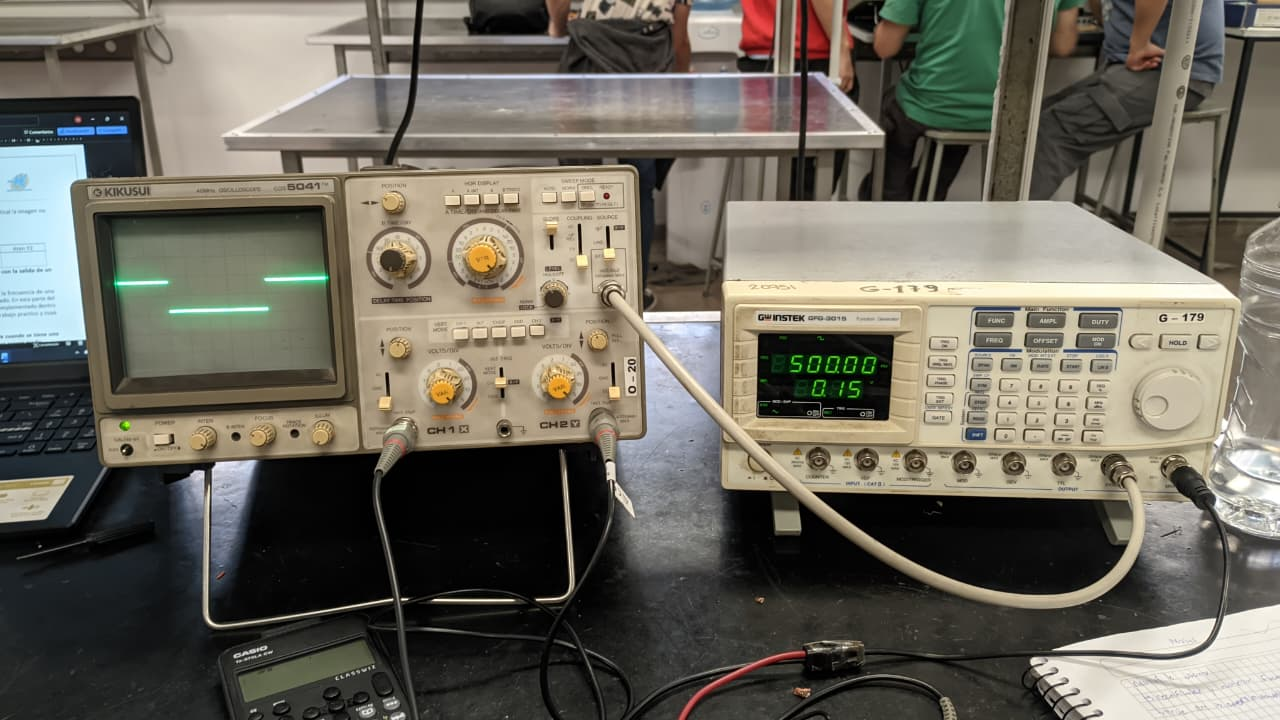
\includegraphics[width=0.4\textwidth]{images/parte5a.jpeg}
	\caption{Conexión de la salida SYNC del generador al trigger externo del osciloscopio}
	\label{fig:parte5a}
\end{figure} 

\begin{table}[H]
\resizebox{\columnwidth}{!}{%
\begin{tabular}{|l|l|l|l|l|}
\hline
V/div (Y1)                & V/div (Y2)               & T/div & Aten Y1                  & Aten Y2                  \\ \hline
\multicolumn{1}{|c|}{50mV} & \multicolumn{1}{c|}{50mV} & 0.2ms & \multicolumn{1}{c|}{x10} & \multicolumn{1}{c|}{x10} \\ \hline
\end{tabular}%
}
\end{table}

Veremos que ahora por mas que variemos la escala de amplitud, la señal no se perderá, a diferencia de antes que se perdía en 1V/div.

\section{Desarrollo Experimental 6}

En esta parte usaremos el modo x-y del osciloscopio para medir la frecuencia de una determinada señal usando como referencia el “Generador de funciones GFG 3015 (B)” 

La señal que queremos medir es la proporcionada por el generador de funciones incluido en la fuente que usamos anteriormente, cuya Frecuencia nominal es de 300 Hz.
Cabe aclarar que esta medición solo se puede realizar si se tiene una idea bastante aproximada de cuál es la frecuencia de la señal a medir.
Ahora procedemos a conectar la salida del generador que tiene la fuente al canal 1 del osciloscopio y medimos la amplitud de la señal.


\begin{figure}[H]
    \centering
    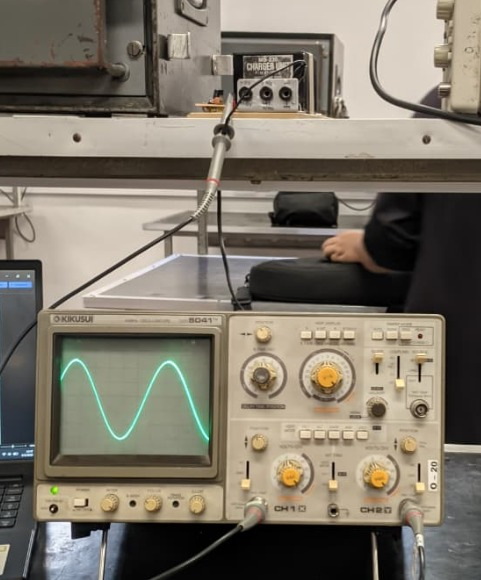
\includegraphics[width=0.4\textwidth]{images/parte6a0.jpeg}
    \caption{Señal del generador de funciones de la fuente}
    \label{fig:parte6}
\end{figure}

\begin{table}[H]
    \centering
\resizebox{0.6\columnwidth}{!}{%
\begin{tabular}{|c|c|c|}
\hline
\textbf{Frec(Nominal)} & \textbf{Función} & \textbf{Amplitud} \\ \hline
300 Hz              & Senoidal         & 11Vpp              \\ \hline
\end{tabular}%
}
\end{table}

Ahora conectamos la salida del generador de funciones GFG 3015 al canal 2 del osciloscopio, ajustamos los valores de amplitud y frecuencia iguales a los de la señal de la fuente.
\begin{figure}[H]
    \centering
    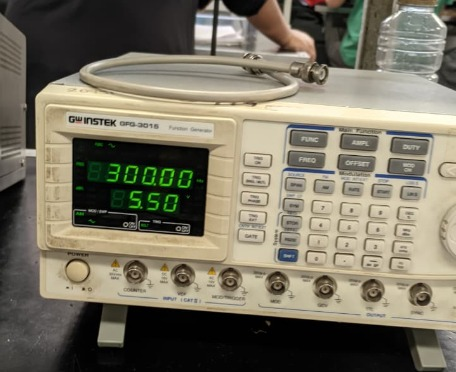
\includegraphics[width=0.4\textwidth]{images/6ach2.jpeg}
    \caption{Generador de funciones GFG 3015 configurado}
    \label{fig:parte6a}
\end{figure}

Ahora ponemos el osciloscopio en modo x-y y observamos que la figura que se forma no es estable y se mueve constantemente. Eso quiere decir que la frecuencia de la señal del canal 1 no es exactamente la frecuencia de 300Hz que pensamos anteriormente, sino que es un poco diferente y por eso la figura se ve inestable. Para estabilizar la figura, ajustamos la frecuencia del generador de funciones GFG 3015 hasta que la figura se vea estable. De esta forma, podemos medir la frecuencia de la señal del canal 1 con mayor precisión. Lo que se logra ver al estabilizar la figura es lo siguiente:

\begin{figure}[H]
    \centering
    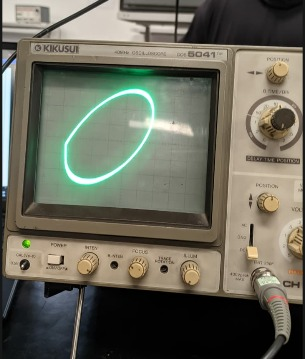
\includegraphics[width=0.4\textwidth]{images/parte6a.jpeg}
    \caption{Figura estable en modo x-y}
    \label{fig:parte6}
\end{figure}

La frecuencia que se obtiene al ajustar el generador de funciones GFG 3015 es de:

\begin{figure}[H]
    \centering
    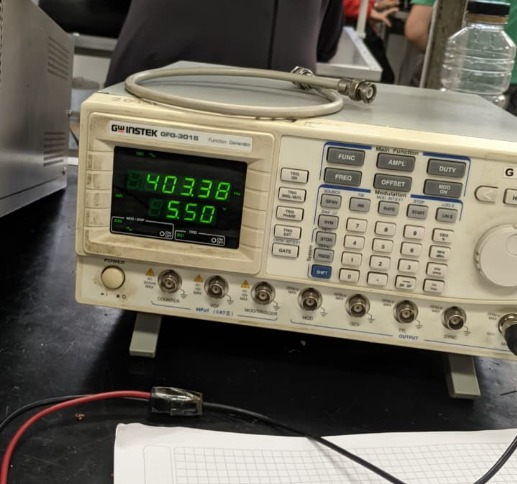
\includegraphics[width=0.4\textwidth]{images/parte6b.jpeg}
    \caption{Frecuencia ajustada del generador de funciones GFG 3015}
    \label{fig:parte6b}
\end{figure}

Por lo tanto concluimos que la frecuencia de la señal del canal 1 es de aproximadamente \textbf{Frecuencia}: 403.38Hz.

\section{Desarrollo Experimental 7}

Para esta parte haremos uso del generador de funciones GF3015 y lo condiguraremos con los siguientes datos:

\begin{table}[H]
\resizebox{\columnwidth}{!}{%
\begin{tabular}{|c|c|c|c|c|c|}
\hline
\textbf{Frec.} & \textbf{Func.} & \textbf{Ampl.} & \textbf{Duty} & \textbf{Trig.} & \textbf{Trig. Ext.} \\ \hline
2KHz           & Cuadr.         & 5Vpp           & 50\%          & Mult.          & Desact.             \\ \hline
\end{tabular}%
}
\end{table}

\begin{table}[H]
\resizebox{\columnwidth}{!}{%
\begin{tabular}{|c|c|c|c|c|}
\hline
\textbf{Rate} & \textbf{Sym.} & \textbf{Trig. Phase} & \textbf{Source} & \textbf{Trig. on/off} \\ \hline
0.5KHz        & 50\%          & 30\%                 & Triang.         & on                    \\ \hline
\end{tabular}%
}
\end{table}

Ahora conectaremos al osciloscopio y pondremos la base de tiempo entre 1ms/div y 0.1ms/div, veremos lo siguiente:

\begin{figure}[H]
	\centering
    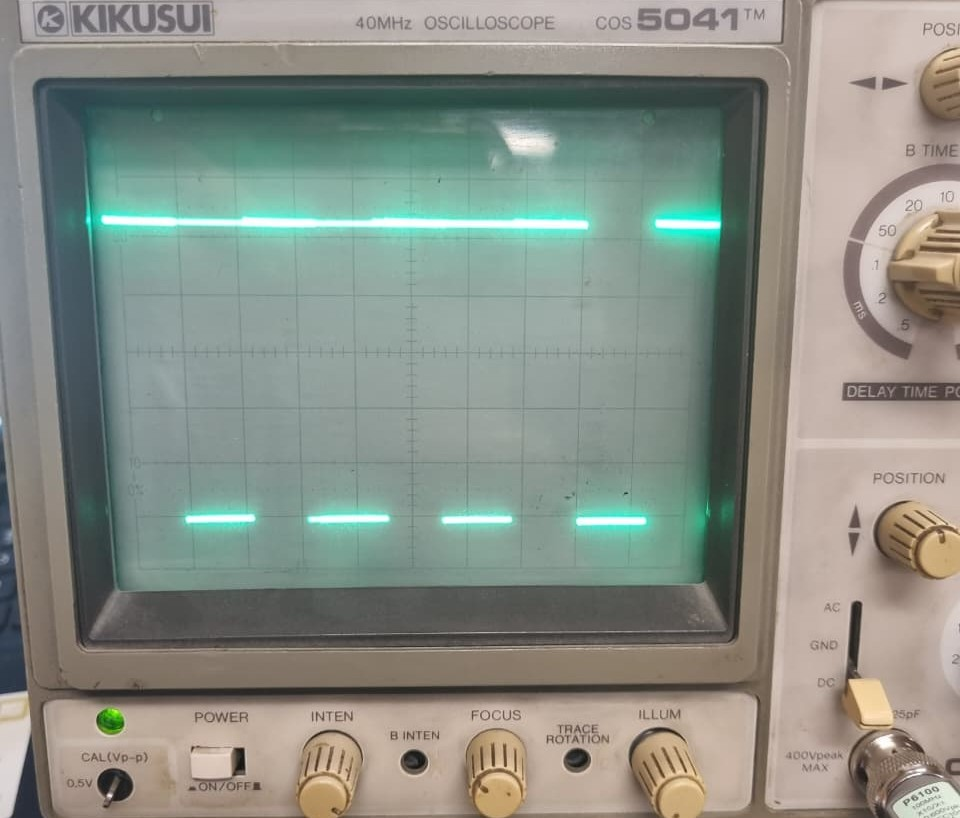
\includegraphics[width=0.4\textwidth]{images/parte7a.jpeg}
    \caption{Superposición de señales}
    \label{fig:parte7a}
\end{figure}

Se ven dos imagenes solapadas entre sí, una siendo la parte ancha del tren de pulsos y la otra siendo la parte angosta, para ver esto con mayor claridad, vamosa ajustar el Holf-of y el Nivel de disparo para llegar a lo siguiente:

\begin{figure}[H]
	\centering
    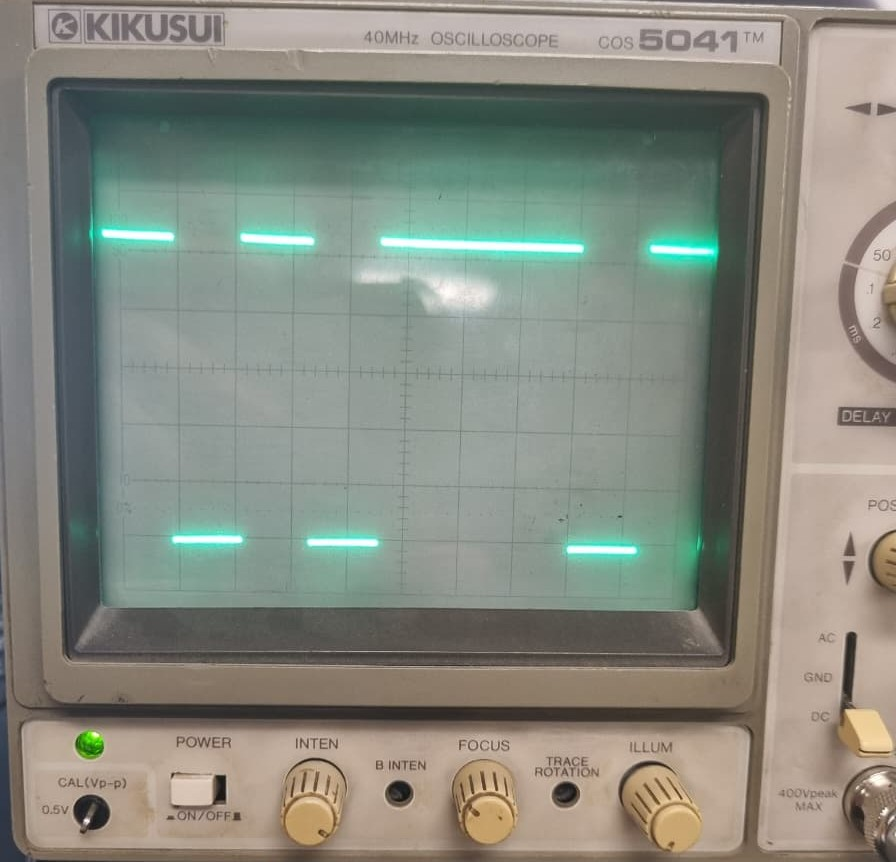
\includegraphics[width=0.4\textwidth]{images/parte7b.jpeg}
    \caption{Señal en de tren de pulsos}
    \label{fig:parte7b}
\end{figure}

\begin{table}[H]
\resizebox{\columnwidth}{!}{%
\begin{tabular}{|l|l|l|l|l|}
\hline
V/div (Y1)                & V/div (Y2)               & T/div & Aten Y1                  & Aten Y2                  \\ \hline
\multicolumn{1}{|c|}{0.1V} & \multicolumn{1}{c|}{0.1V} & 0.2ms & \multicolumn{1}{c|}{x10} & \multicolumn{1}{c|}{x10} \\ \hline
\end{tabular}%
}
\end{table}

\section{Desarrollo Experimental 8}

Ahora tal cual y como dejamos todos, usaremos el Doble Trazo, para ello usando solo el canal 1, conectaremos al canal 2 al generador en la parte de ''MOD''. Activamos el doble trazo en modo ''ALTERNADO'', y ajustamos la amplitud para ver una imagen adecuada.

\begin{figure}[H]
	\centering
    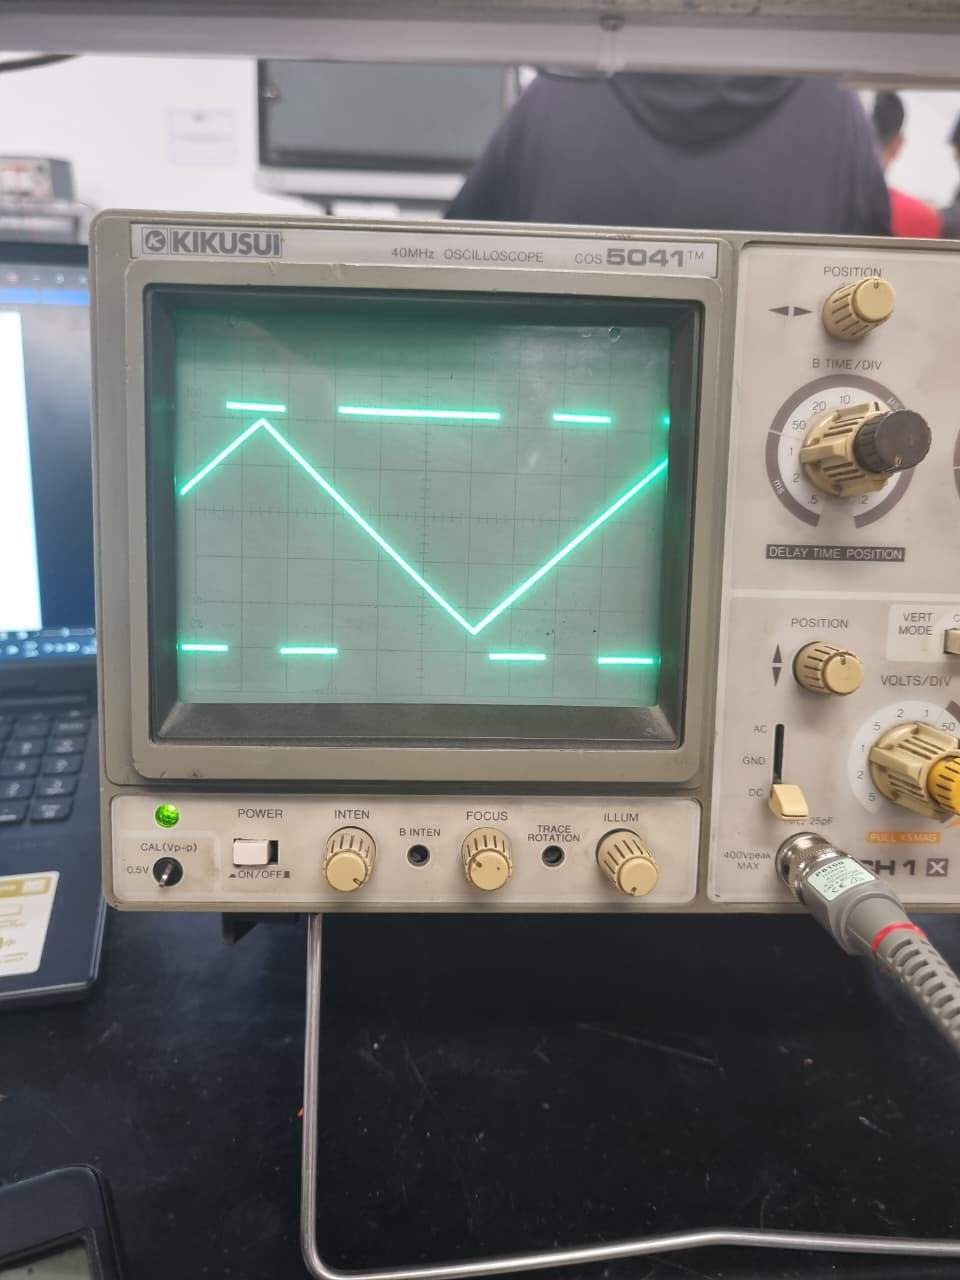
\includegraphics[width=0.4\textwidth]{images/parte8a.jpeg}
    \caption{Señales en modo alternado}
    \label{fig:parte8a}
\end{figure}

Ahora calculamos los siguientes datos:

\begin{table}[H]
\resizebox{\columnwidth}{!}{%
\begin{tabular}{|l|l|l|l|l|}
\hline
V/div (Y1)                & V/div (Y2)               & T/div & Aten Y1                  & Aten Y2                  \\ \hline
\multicolumn{1}{|c|}{0.1V} & \multicolumn{1}{c|}{1V} & 0.2ms & \multicolumn{1}{c|}{x10} & \multicolumn{1}{c|}{x10} \\ \hline
\end{tabular}%
}
\end{table}

Grafica de ambas señales: